\documentclass[14pt]{article}

\usepackage[utf8]{inputenc}
\usepackage[russian]{babel}

\usepackage{setspace}
\setstretch{1.5}

\usepackage{indentfirst}
\setlength{\parindent}{1.25cm}

\usepackage{float}
\usepackage{geometry}
\usepackage{graphicx}
\usepackage{tocloft}
\usepackage{hyperref}
\usepackage{enumitem}
\usepackage{csvsimple}

\graphicspath{ {./img/} }

\renewcommand{\cftsecleader}{\cftdotfill{\cftdotsep}}
\addto\captionsrussian{\def\refname{Список использованных источников}}

\begin{document}
\newgeometry{left=30mm, top=20mm, right=15mm, bottom=20mm, nohead}
\begin{titlepage}
\begin{center}
{\Large Санкт--Петербургский государственный университет} \\
Направление: 01.03.02 «Прикладная математика и информатика» \\
ООП: Прикладная математика, фундаментальная информатика и программирование
\vspace{55mm} \\
\textbf{\large ОТЧЕТ О НАУЧНО-ИССЛЕДОВАТЕЛЬСКОЙ ПРАКТИКЕ} \\ [10mm]
{\large }
\begin{flushleft}
{\large \textbf{Тема задания :} Разработка системы распознавания речевых команд при помощи методов машинного обучения} \\ [5mm]
{\large \textbf{Выполнил :} Мирошниченко Александр Сергеевич  группа 17.Б05} \\[5mm]
{\large \textbf{Руководитель практики от СПбГУ :} Козынченко В. А., кандидат физ.-мат. наук, доцент} \\[5mm]
\end{flushleft}
\vfill 
{Санкт-Петербург}
\par{2021 г.}
\end{center}
\end{titlepage}
\addtocounter{page}{1}

\tableofcontents
\newpage

\addcontentsline{toc}{section}{Введение}
\section*{Введение}
Распознавание речи является одной из важнейших задач взаимодействия человека и компьютера на сегодняшний день. Одним из способов решения задачи распознавания речи является ввод информации в вычислительное устройство при помощи микрофона; далее происходит преобразование звуковых колебаний в электрический сигнал, оцифровываемый компьютером и записываемый в определенный звуковой формат в виде набора числовых данных. Полученное числовое представление преобразованного звукового сигнала можно обрабатывать при помощи алгоритма для достижения поставленных целей. Одной из таких целей является преобразование в текст - набор слов, произнесенных человеком при записи звука в микрофон и последующее выполнение компьютером или исполнительными устройствами действий, согласно заданным условиям соответствия действия и полученного слова-команды. \\

    Данная проблема была актуальна с времен появления компьютеров и остается таковой и по сей день. Изначально для решения данной задачи применялись такие алгоритмы, как скрытые Марковские модели, методы динамического программирования, методы дискриминантного анализа, основанные на Байесовской дискриминации и другие. В последнее время стали актуальны методы, основанные на нейронных сетях. С ростом вычислительной мощности компьютеров стало возможным выполнение большего количества математических операций и популярность нейронных сетей, требующих такой мощности, растет. 

\addcontentsline{toc}{section}{Постановка задачи}
\section*{Постановка задачи}
Разработать и запрограммировать алгоритм распознавания звуковых команд в виде отдельных слов при помощи нейронной сети.

\addcontentsline{toc}{section}{Выбор инструментов для решения задачи}
\section*{Выбор инструментов для решения задачи}
Для решения задачи был выбран язык программирования Python 3.8. Предобработку данных было решено реализовывать при помощи Python 3.8.
В качестве библиотеки для реализации нейронной сети была выбрана библиотека Keras, включенная в библиотеку Tensorflow 2.4.1. \\

Для создания датасета был разработан веб-сервис на NodeJS, Javascript, HTML, CSS, который позволяет записывать команды и сохранять их в нужном для программы предобработки формате. Также это позволило записать необходимое количество дикторов, которые смогли довольно быстро наговорить команды.
\newpage

\addcontentsline{toc}{section}{Результаты вычислений}
\section*{Результаты вычислений}
Было проведено 3 вычислительных эксперимента для нейронной сети типа CNN. Структура сети приведена на рисунке \ref{fig:cnn_model}.

\begin{figure}[H]
  \[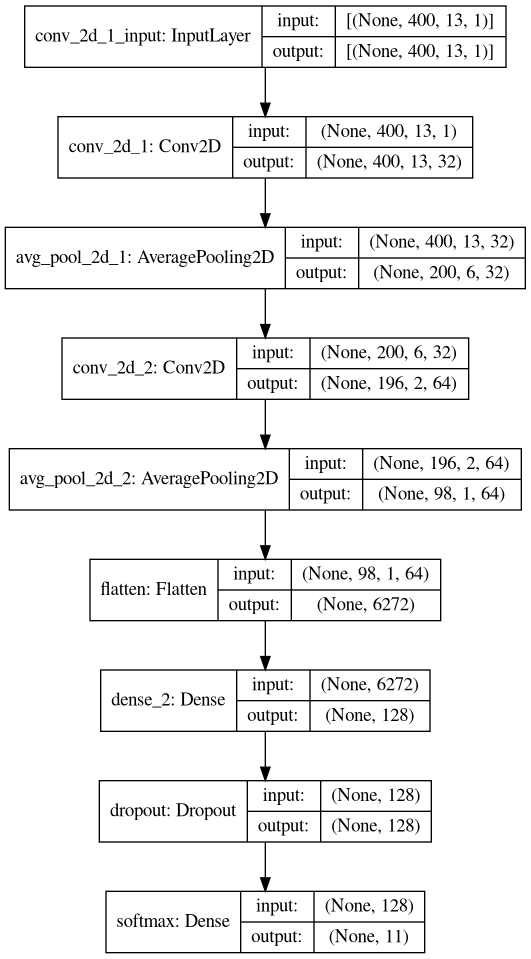
\includegraphics[scale=0.4]{cnn_model.png}\]
  \caption{Структура модели нейронной сети типа CNN}
  \label{fig:cnn_model}
\end{figure}

Все звуковые файлы были предобработаны при помощи алгоритма MFCC.
Звуковая дорожка делится на фреймы. Каждый фрейм - отрезок звуковой дорожки длительностью 20 мс. Каждый фрейм начинается с момента (10 мс. $\times$ номер\_фрейма), нумерация начинается с 0. Для каждой звуковой дорожки количество фреймов - 400. Если количество фреймов у дорожки меньше 400, то слева и справа добавляются нули. Это число было выбрано как максимально возможное количество фреймов для всех дорожек. Количество коэффициентов в алгоритме MFCC - 13, количество фильтров - 26. В итоге размерность данных, поступающих на вход нейронной сети - $400\times13$.

Датасет состоит из 6 дикторов. Каждый диктор записал 11 команд : 'back', 'down', 'menu', 'off', 'on', 'open', 'play', 'power', 'stop', 'up', 'volume'.
\\

\begin{tabular}[c]{ | p{2cm} | p{2cm} | p{6cm} | p{4cm} | }
\hline
Диктор & Тип голоса & Кол-во звук. дорожек на каждую команду & Сумм. кол-во звук. дорожек  \\ \hline
speaker1 & Мужской & 50 & 550 \\
speaker2 & Мужской & 40 & 440 \\
speaker3 & Мужской & 40 & 440 \\
speaker4 & Мужской & 40 & 440 \\
speaker5 & Мужской & 50 & 550 \\
speaker6 & Женский & 50 & 550 \\ \hline
\end{tabular}
\\

Первый эксперимент: нейронная сеть обучается на первом дикторе с мужским голосом, тестирование производится на каждом дикторе. 

Второй эксперимент: нейронная сеть обучается на всех дикторах с мужским голосом, тестирование производится на каждом дикторе. 

Третий эксперимент: нейронная сеть обучается на всех дикторах, тестирование производится на каждом дикторе.

Датасет предварительно разделяется на тренировочную и тестовую части. На тренировочную часть отводится 70\% данных диктора, на тестовую часть - 30\%. В процессе тренировки после каждой эпохи тренировочные данные перемешиваются. 15\% тренировочных данных в каждой эпохе - валидационные. В качестве метрики для оценки эффективности была выбрана метрика точности (accuracy), а для валидации - функция потерь категориальной кросс-энтропии (val\_loss). Алгоритм оптимизации - Adam. Максимальное количество эпох - 50. Если значение метрики val\_loss не уменьшается в течение 20 эпох, то обучение останавливается.

Графики обучения для каждого из экспериментов приведены на рисунках \ref{fig:cnn_speaker1_train_graphs}, \ref{fig:cnn_all_male_speakers_train_graphs}, \ref{fig:cnn_all_speakers_train_graphs}.

В конце каждого эксперимента проводится тестирование нейронной сети.
А в случае обучения на all\_speakers помимо тестирования производится построение матрицы ошибок (confusion matrix) для каждого диктора и для каждого из четырех пороговых значений: 0.5, 0.6, 0.7, 0.8. Матрицы представлены на рисунке \ref{fig:cnn_cm_all_speakers}.

Результаты тестирования представлены в таблице \ref{table:test_summary}. Обозначения, которые используются:

all\_speakers = [speaker1, speaker2, speaker3, speaker4, speaker5, speaker6]

all\_male\_speakers = [speaker1, speaker2, speaker3, speaker4, speaker5]

\begin{figure}[H]
  \[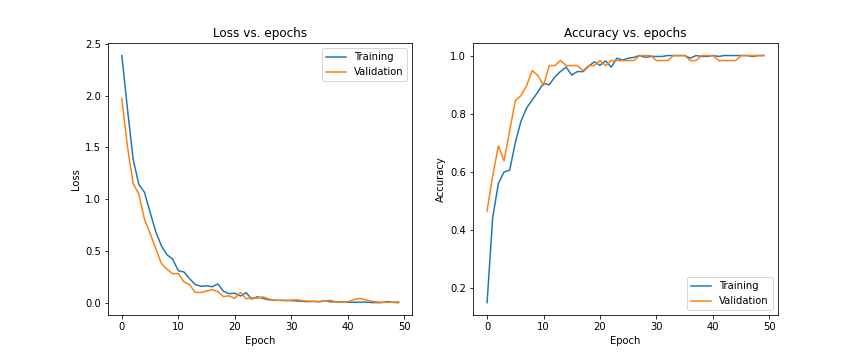
\includegraphics[scale=0.4]{cnn_speaker1_train_graphs.png}\]
  \caption{Графики функции потерь и точности в течение обучения на speaker1}
  \label{fig:cnn_speaker1_train_graphs}
\end{figure}

\begin{figure}[H]
  \[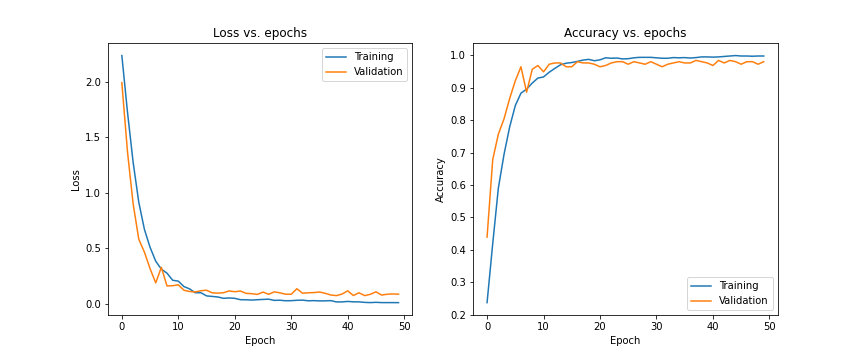
\includegraphics[scale=0.4]{cnn_all_male_speakers_train_graphs.png}\]
  \caption{Графики функции потерь и точности в течение обучения на all\_male\_speakers}
  \label{fig:cnn_all_male_speakers_train_graphs}
\end{figure}

\begin{figure}[H]
  \[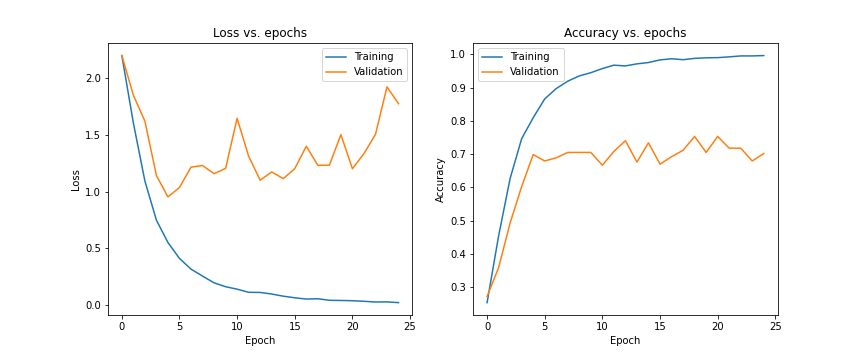
\includegraphics[scale=0.4]{cnn_all_speakers_train_graphs.png}\]
  \caption{Графики функции потерь и точности в течение обучения на all\_speakers}
  \label{fig:cnn_all_speakers_train_graphs}
\end{figure}


\begin{table}
\centering
\csvautotabular[respect underscore=true]{test_summary.csv}
\caption{Результаты вычислений}
\label{table:test_summary}
\end{table}

\begin{figure}[H]
  \[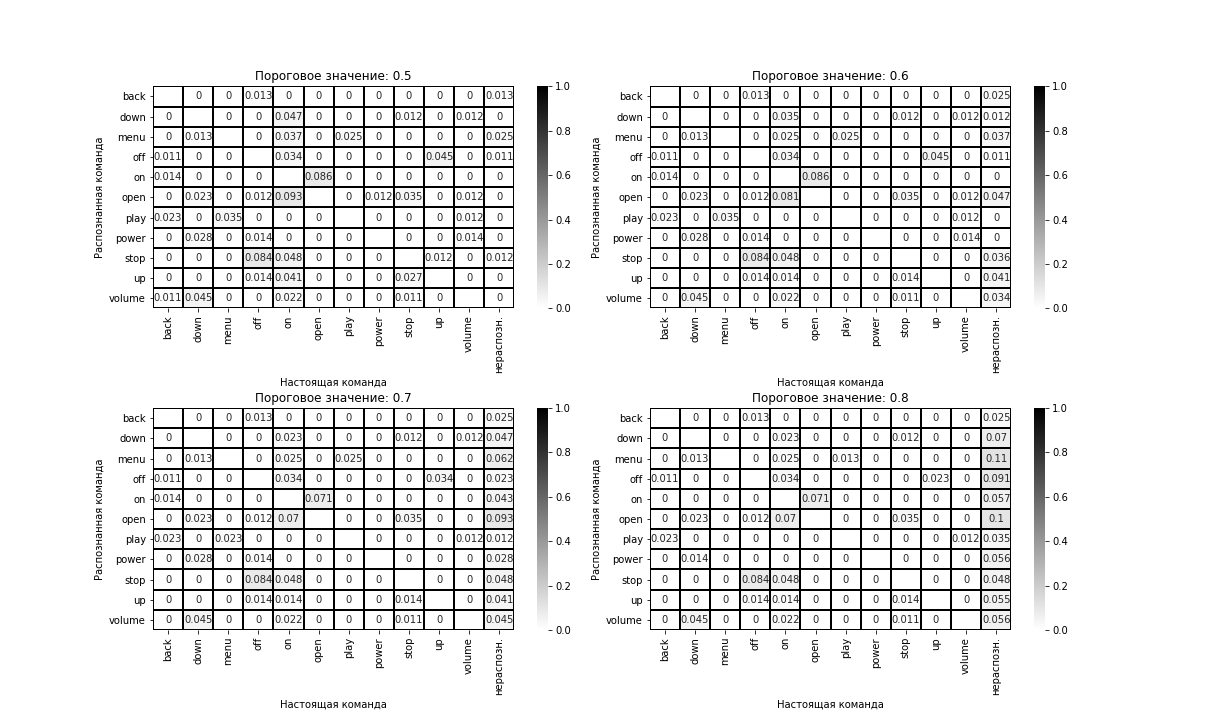
\includegraphics[scale=0.4]{cnn_cm_all_speakers.png}\]
  \caption{Матрицы ошибок для случая обучения на all\_speakers}
  \label{fig:cnn_cm_all_speakers}
\end{figure}

Видно, что при обучении только на одном дикторе, распознавание на всех остальных работает плохо. 

При обучении только на мужских голосах, распознавание на женском работает лучше, чем при обучении на одном, но все-равно очень плохо.

При обучении на всех голосах, распознавание на каждом голосе дает приемлемую точность. Однако стоит отметить, что если большая часть голосов в тренировочной части - мужские, то на женском голосе распознавание будет работать хуже, чем на мужских.

\addcontentsline{toc}{section}{Заключение}
\section*{Заключение}
В данной работе:
\begin{itemize}[leftmargin=2cm]
\item Проведена предобработка звуковых дорожек, содержащих команды в wav файлах
\item Разработан алгоритм распознавания речевых команд
\item Реализован алгоритм распознавания речевых команд
\item Проведены вычислительные эксперименты, в результате которых	 показана работоспособность и эффективность работы алгоритма распознавания речевых команд.
\end{itemize}
\newpage

\addcontentsline{toc}{section}{Список использованных источников}
\begin{thebibliography}{3}
\bibitem{Aurélien2019}
Aurélien G. Hands-On Machine Learning with Scikit-Learn, Keras, and TensorFlow: Concepts, Tools, and Techniques to Build Intelligent Systems / Aurélien G. --- 2nd Edition --- O'Reilly Media, 2019.
\bibitem{DeepLearningArticle}
Hendrik Purwins, Bo Li, Tuomas Virtanen, Jan Schlüter, Shuo-yiin Chang, Tara Sainath Deep Learning for Audio Signal Processing // Journal  of  Selected  Topics  of  Signal  Processing,  Vol.  13,  No.  2,  May  2019, pages 206–219.
\bibitem{TensorFlowDocs}
Документация TensorFlow [Электронный ресурс]. --- Режим доступа: https://www.tensorflow.org/api\_docs/python/tf
\bibitem{MLportal}
Портал ML Glossary [Электронный ресурс]. --- Режим доступа: https://ml-cheatsheet.readthedocs.io
\bibitem{CourseraCourse}
Курс на платформе Coursera [Электронный ресурс]. --- Режим доступа: https://www.coursera.org/learn/getting-started-with-tensor-flow2
\bibitem{FourierTransformWiki}
Страница на Википедии [Электронный ресурс]. --- Режим доступа: https://en.wikipedia.org/wiki/Fourier\_transform
\bibitem{MelScaleWiki}
Страница на Википедии [Электронный ресурс]. --- Режим доступа: https://en.wikipedia.org/wiki/Mel\_scale

\end{thebibliography}
\newpage

\addcontentsline{toc}{section}{Приложение}
\section*{Приложение}
Ссылка на репозиторий с программой веб-сервисом для записи датасета, состоящего из звуковых файлов: \url{https://gitlab.com/polotent/commandrecorder} \\

Ссылка на репозиторий c программой предобработки данных, обучением и тестированием нейронной сети: \url{https://gitlab.com/polotent/boxy}
\restoregeometry

\end{document}